%%\documentclass[a4paper,12pt,oneside]{llncs}
\documentclass[12pt,letterpaper]{article}
\usepackage[right=2cm,left=3cm,top=2cm,bottom=2cm,headsep=0cm]{geometry}

%%%%%%%%%%%%%%%%%%%%%%%%%%%%%%%%%%%%%%%%%%%%%%%%%%%%%%%%%%%
%% Juego de caracteres usado en el archivo fuente: UTF-8
\usepackage{ucs}
\usepackage[utf8x]{inputenc}

%%%%%%%%%%%%%%%%%%%%%%%%%%%%%%%%%%%%%%%%%%%%%%%%%%%%%%%%%%%
%% Juego de caracteres usado en la salida dvi
%% Otra posibilidad: \usepackage{t1enc}
\usepackage[T1]{fontenc}

%%%%%%%%%%%%%%%%%%%%%%%%%%%%%%%%%%%%%%%%%%%%%%%%%%%%%%%%%%%
%% Ajusta maergenes para a4
%\usepackage{a4wide}

%%%%%%%%%%%%%%%%%%%%%%%%%%%%%%%%%%%%%%%%%%%%%%%%%%%%%%%%%%%
%% Uso fuente postscript times, para que los ps y pdf queden y pequeños...
\usepackage{times}

%%%%%%%%%%%%%%%%%%%%%%%%%%%%%%%%%%%%%%%%%%%%%%%%%%%%%%%%%%%
%% Posibilidad de hipertexto (especialmente en pdf)
%\usepackage{hyperref}
\usepackage[bookmarks = true, colorlinks=true, linkcolor = black, citecolor = black, menucolor = black, urlcolor = black]{hyperref}

%%%%%%%%%%%%%%%%%%%%%%%%%%%%%%%%%%%%%%%%%%%%%%%%%%%%%%%%%%%
%% Graficos 
\usepackage{graphics,graphicx}

%%%%%%%%%%%%%%%%%%%%%%%%%%%%%%%%%%%%%%%%%%%%%%%%%%%%%%%%%%%
%% Ciertos caracteres "raros"...
\usepackage{latexsym}

%%%%%%%%%%%%%%%%%%%%%%%%%%%%%%%%%%%%%%%%%%%%%%%%%%%%%%%%%%%
%% Matematicas aun más fuertes (american math dociety)
\usepackage{amsmath}

%%%%%%%%%%%%%%%%%%%%%%%%%%%%%%%%%%%%%%%%%%%%%%%%%%%%%%%%%%%
\usepackage{multirow} % para las tablas
\usepackage[spanish,es-tabla]{babel}

%%%%%%%%%%%%%%%%%%%%%%%%%%%%%%%%%%%%%%%%%%%%%%%%%%%%%%%%%%%
%% Fuentes matematicas lo mas compatibles posibles con postscript (times)
%% (Esto no funciona para todos los simbolos pero reduce mucho el tamaño del
%% pdf si hay muchas matamaticas....
%\usepackage{mathptm}

%%% VARIOS:
%\usepackage{slashbox}
\usepackage{verbatim}
\usepackage{array}
\usepackage{listings}
\usepackage{multirow}

%% MARCA DE AGUA
%% Este package de "draft copy" NO funciona con pdflatex
%%\usepackage{draftcopy}
%% Este package de "draft copy" SI funciona con pdflatex
%%%\usepackage{pdfdraftcopy}
%%%%%%%%%%%%%%%%%%%%%%%%%%%%%%%%%%%%%%%%%%%%%%%%%%%%%%%%%%%
%% Indenteacion en español...
\usepackage[spanish]{babel}
\usepackage[svgnames,x11names,table]{xcolor}
\usepackage{listings}
% Para escribir código en C
% \begin{lstlisting}[language=C]
% #include <stdio.h>
% int main(int argc, char* argv[]) {
% puts("Hola mundo!");
% }
% \end{lstlisting}


\title{Notificador de polen}
\author{Jesús Rodríguez Heras\\Juan Pedro Rodríguez Gracia}

\begin{document}
	
	\maketitle
	\begin{abstract} %Poner esto en todas las prácticas de PCTR
		\begin{center}
			Notificador de polen para las personas alérgicas.
		\end{center}
	\end{abstract}
	\thispagestyle{empty}
	\newpage
	
	\tableofcontents
	\newpage
	
	%%\listoftables
	%%\newpage
	
	%%\listoffigures
	%%\newpage
	
	%%%% REAL WORK BEGINS HERE:
	
	%%Configuracion del paquete listings
	\lstset{language=bash, numbers=left, numberstyle=\tiny, numbersep=10pt, firstnumber=1, stepnumber=1, basicstyle=\small\ttfamily, tabsize=1, extendedchars=true, inputencoding=latin1}


\section{Introducción}
Nuestra aplicación consta de dos programas: \texttt{tareas.py} y \texttt{PolenCiudad.py}.
\begin{itemize}
	\item \texttt{\textbf{tareas.py:}} El comportamiento de este programa se basa en recolectar la información acerca del polen que hay en cada ciudad de \url{https://www.eltiempo.es/polen}. La obtención de datos se realiza periódicamente cada 2 horas y se insertan en un archivo ``.csv'' que se guarda en dropbox.  También genera una gráfica que se mostrará por pantalla para que se pueda ver, de modo general el nivel de polen en el resto de todas las ciudades.
	\item \texttt{\textbf{PolenCiudad.py:}} Este programa se encarga de interactuar directamente con el usuario, el cual introducirá la ciudad por la que está interesado en conocer el nivel de polen. El programa descarga el archivo más reciente de los existentes en dropbox (almacenados por el programa anterior) y le devolverá el nivel de polen (alto, medio o bajo) por consola y, además, lo publicará en twitter (\url{https://twitter.com/MuleSteam})\footnote{Hemos utilizado la misma cuenta de twitter que para la práctica de Mule debido a que ya teníamos las claves y no hemos visto necesario el hecho de cambiar de cuenta, ya que es, solamente, para fines académicos.} para que las personas que sigan la cuenta sepan el nivel de polen que hay en las ciudades que han buscado otros usuarios.
\end{itemize}

\section{Almacenamiento y salida de datos}
A la hora de almacenar y leer los datos obtenidos de \url{https://www.eltiempo.es/polen} en dropbox, lo hacemos mediante la librería oficial de python para dropbox.\\

También se creará una gráfica con el nivel de polen existente por cada provincia como información adicional para el usuario.

\section{Tecnologías utilizadas}
Para esta aplicación hemos utilizado python como lenguaje de programación base. Aparte de ello, hemos usado una cola de mensajes como es RabbitMQ debido a la simple interfaz que aporta a la hora de trabajar con ella.\\

También hemos usado la librería oficial de dropbox para python que permitir la comunicación entre la aplicación y la nube para así poder almacenar los datos que se irán recogiendo cada dos horas (cada minuto en las pruebas) y las lecturas a dichos datos que se harán cuando un usuario de la aplicación consulte acerca del nivel de polen existente en su provincia.

\section{Problemas encontrados}
El problema principal que nos encontramos fue que no podíamos instalar RabbitMQ en nuestros portátiles, los cuales cuentan con el sistema operativo Kali Linux (basado en Debian), por lo que tuvimos que hacer el proyecto en una máquina virtual con Ubuntu.\\

También nos hemos encontrado otros problemas menores a la hora de trabajar con python y con las librerías de dropbox y twitter.

\section{Demostración}
\begin{itemize}
	\item Lanzamos el worker \texttt{tareas.py} con Celery:
\end{itemize}
\begin{center}
	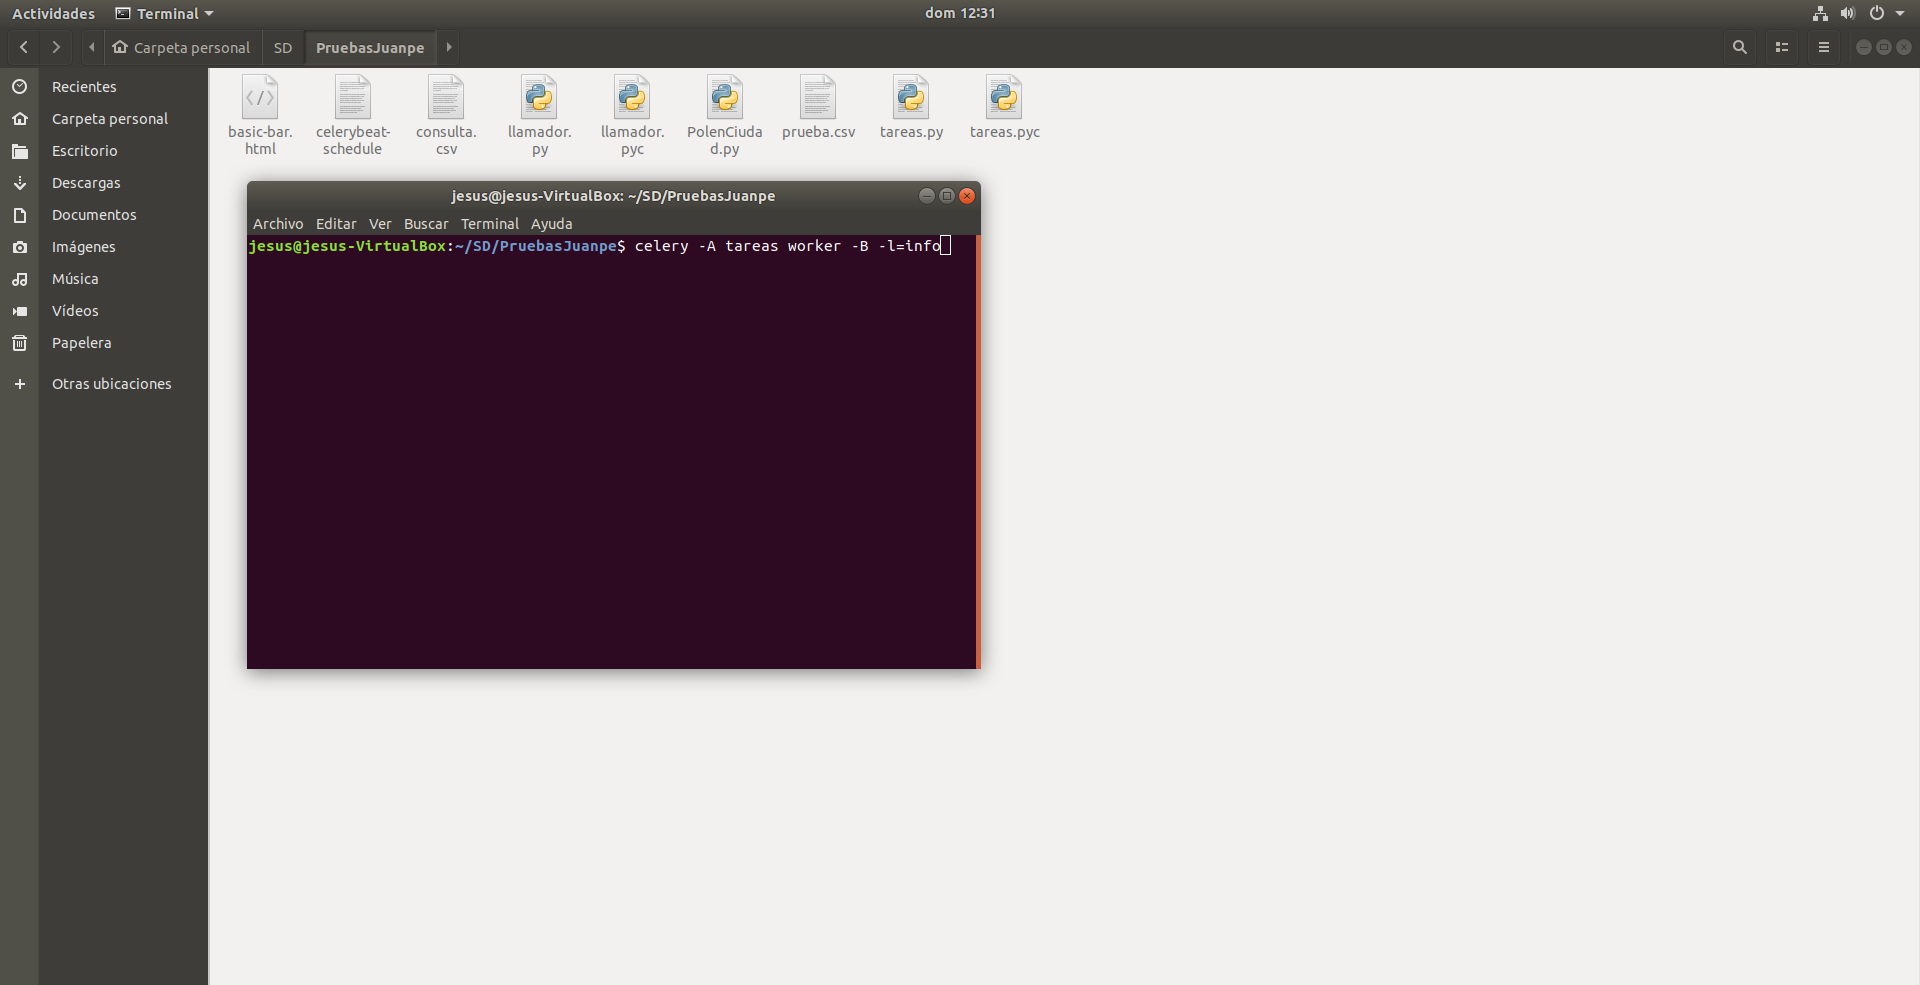
\includegraphics[scale=0.24]{1.png}
\end{center}
\begin{center}
	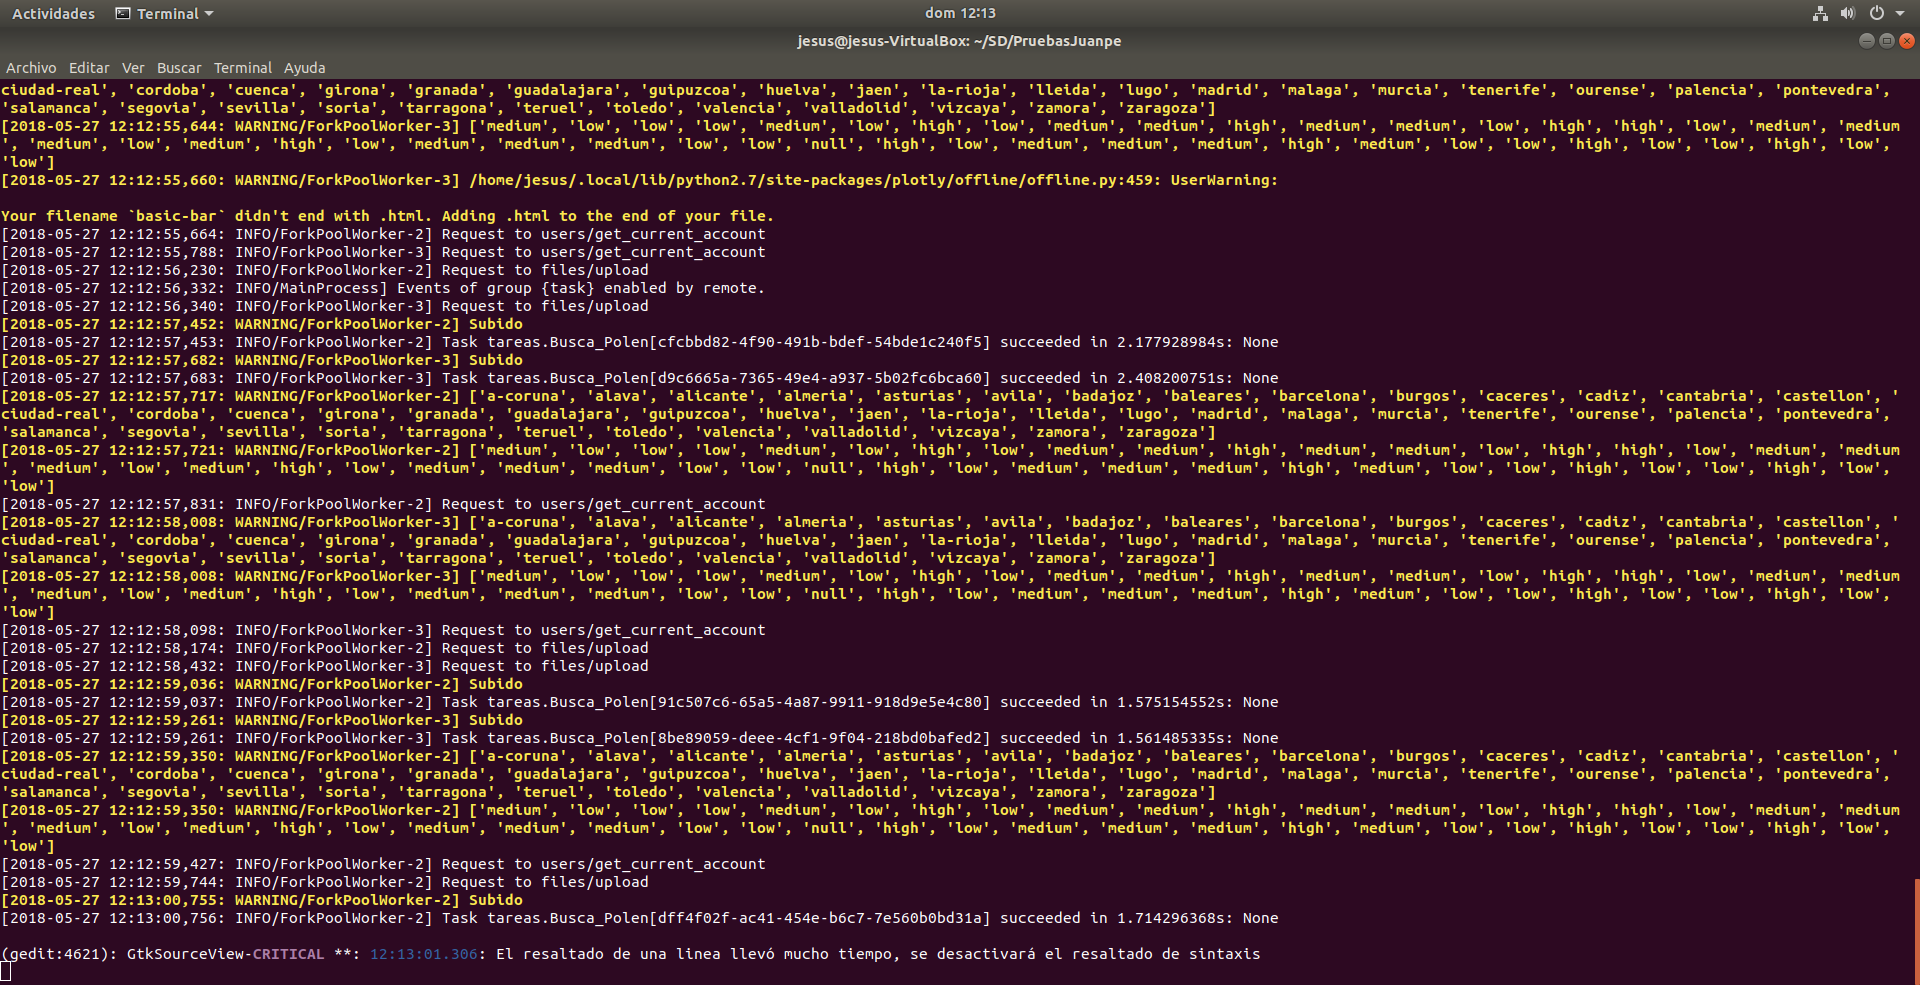
\includegraphics[scale=0.24]{2.png}
\end{center}

\newpage
\begin{itemize}
	\item Se lanzan peticiones a RabbitMQ:
\end{itemize}
\begin{center}
	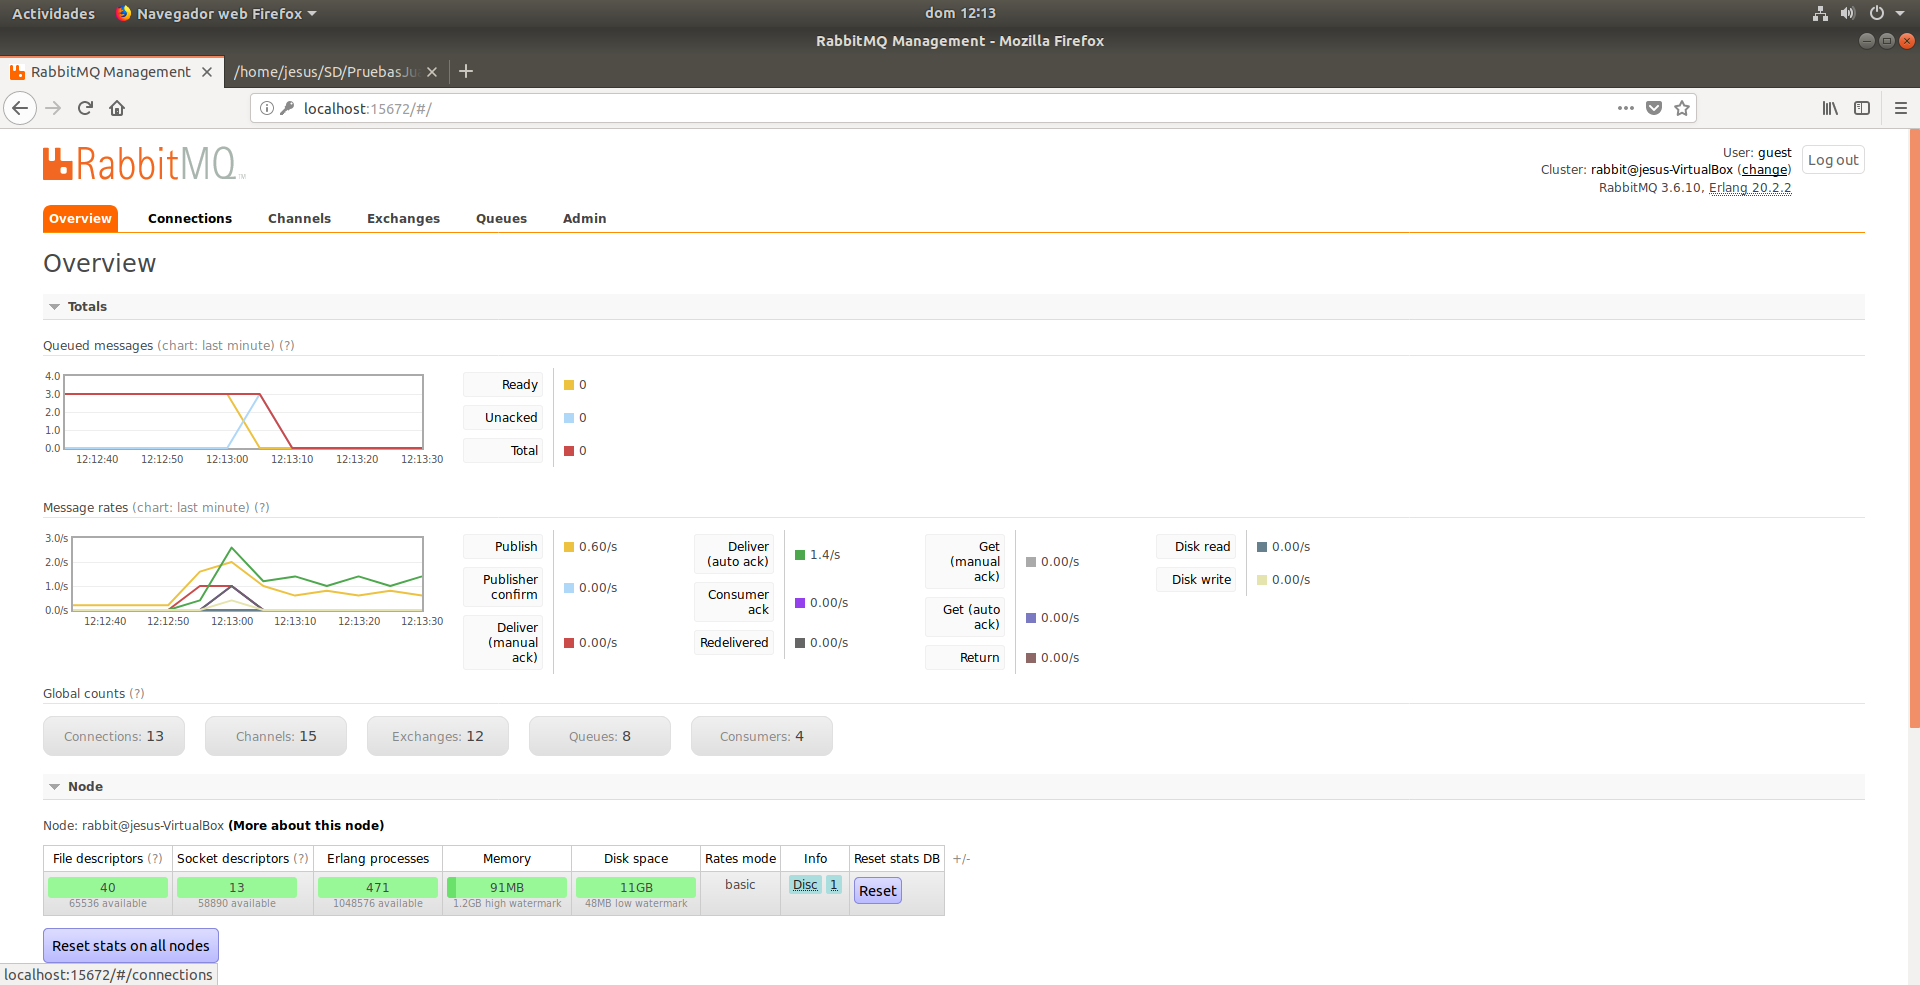
\includegraphics[scale=0.24]{3.png}
\end{center}

\begin{itemize}
	\item También las podemos ver en la interfaz de flower:
\end{itemize}
\begin{center}
	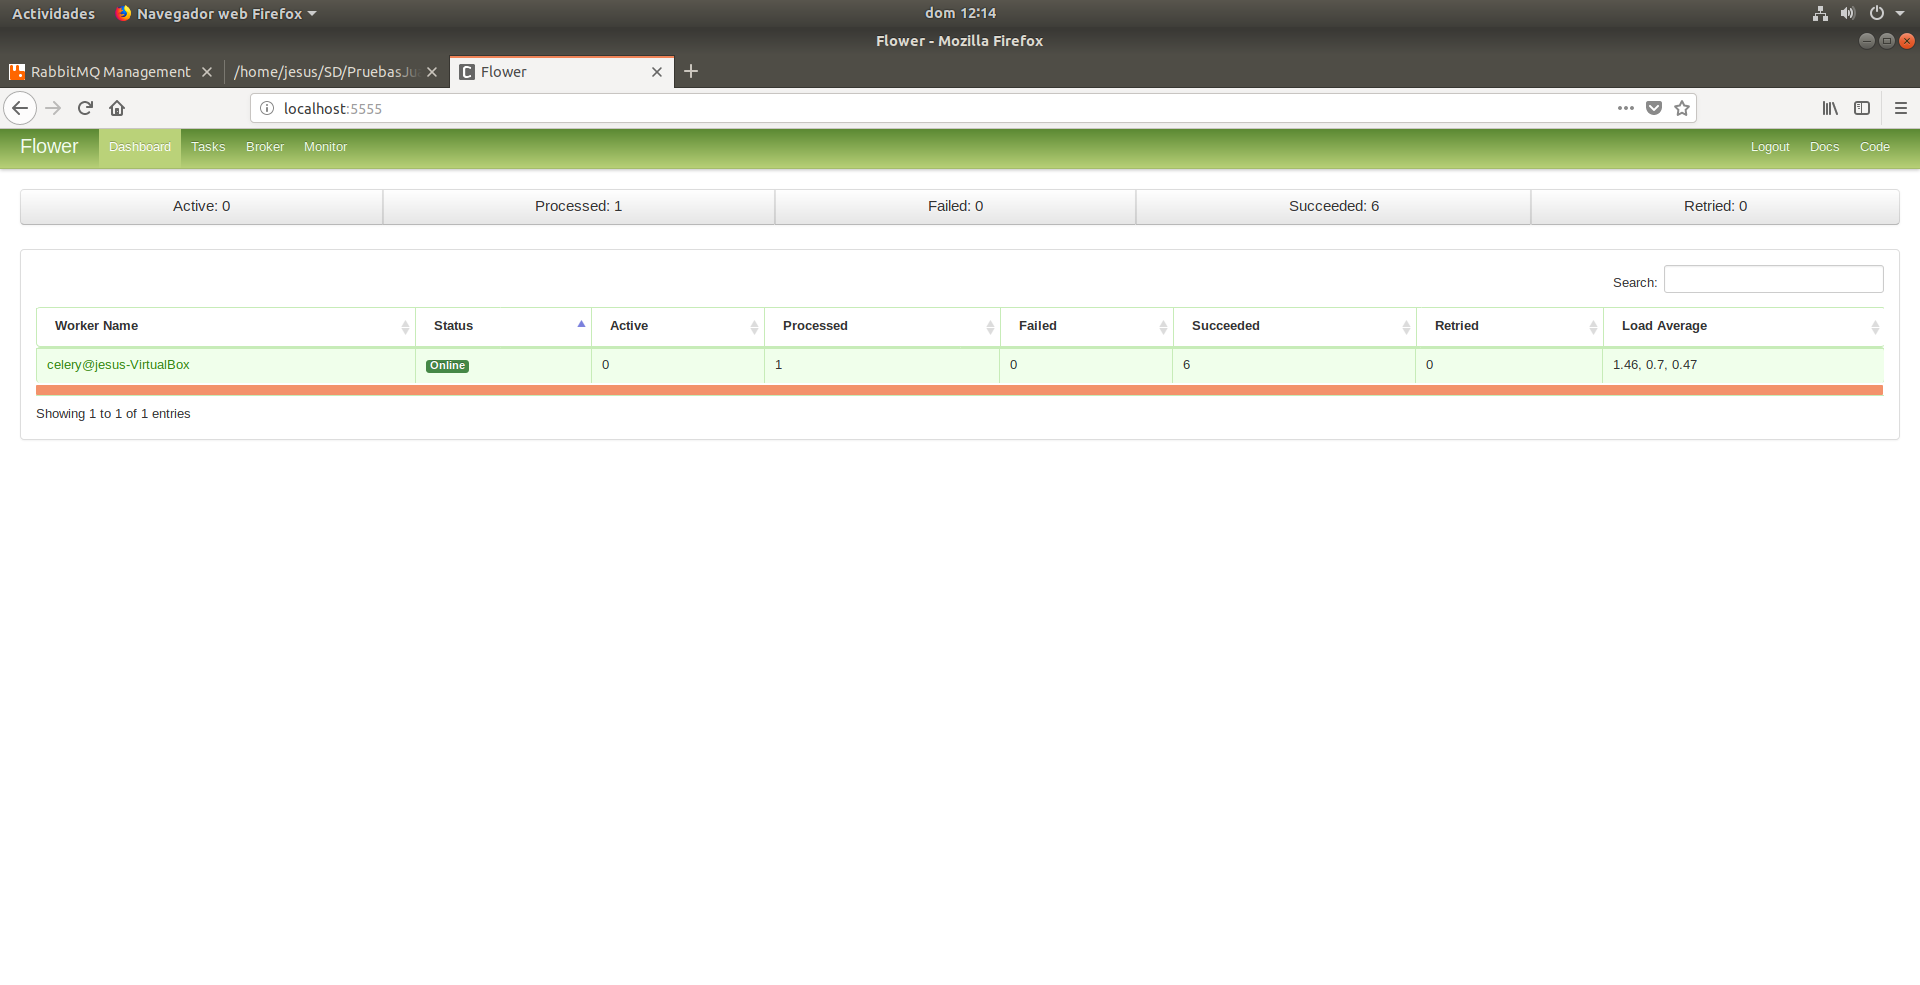
\includegraphics[scale=0.24]{4.png}
\end{center}

\newpage
\begin{itemize}
	\item Gráfica generada por \texttt{tareas.py}:
\end{itemize}
\begin{center}
	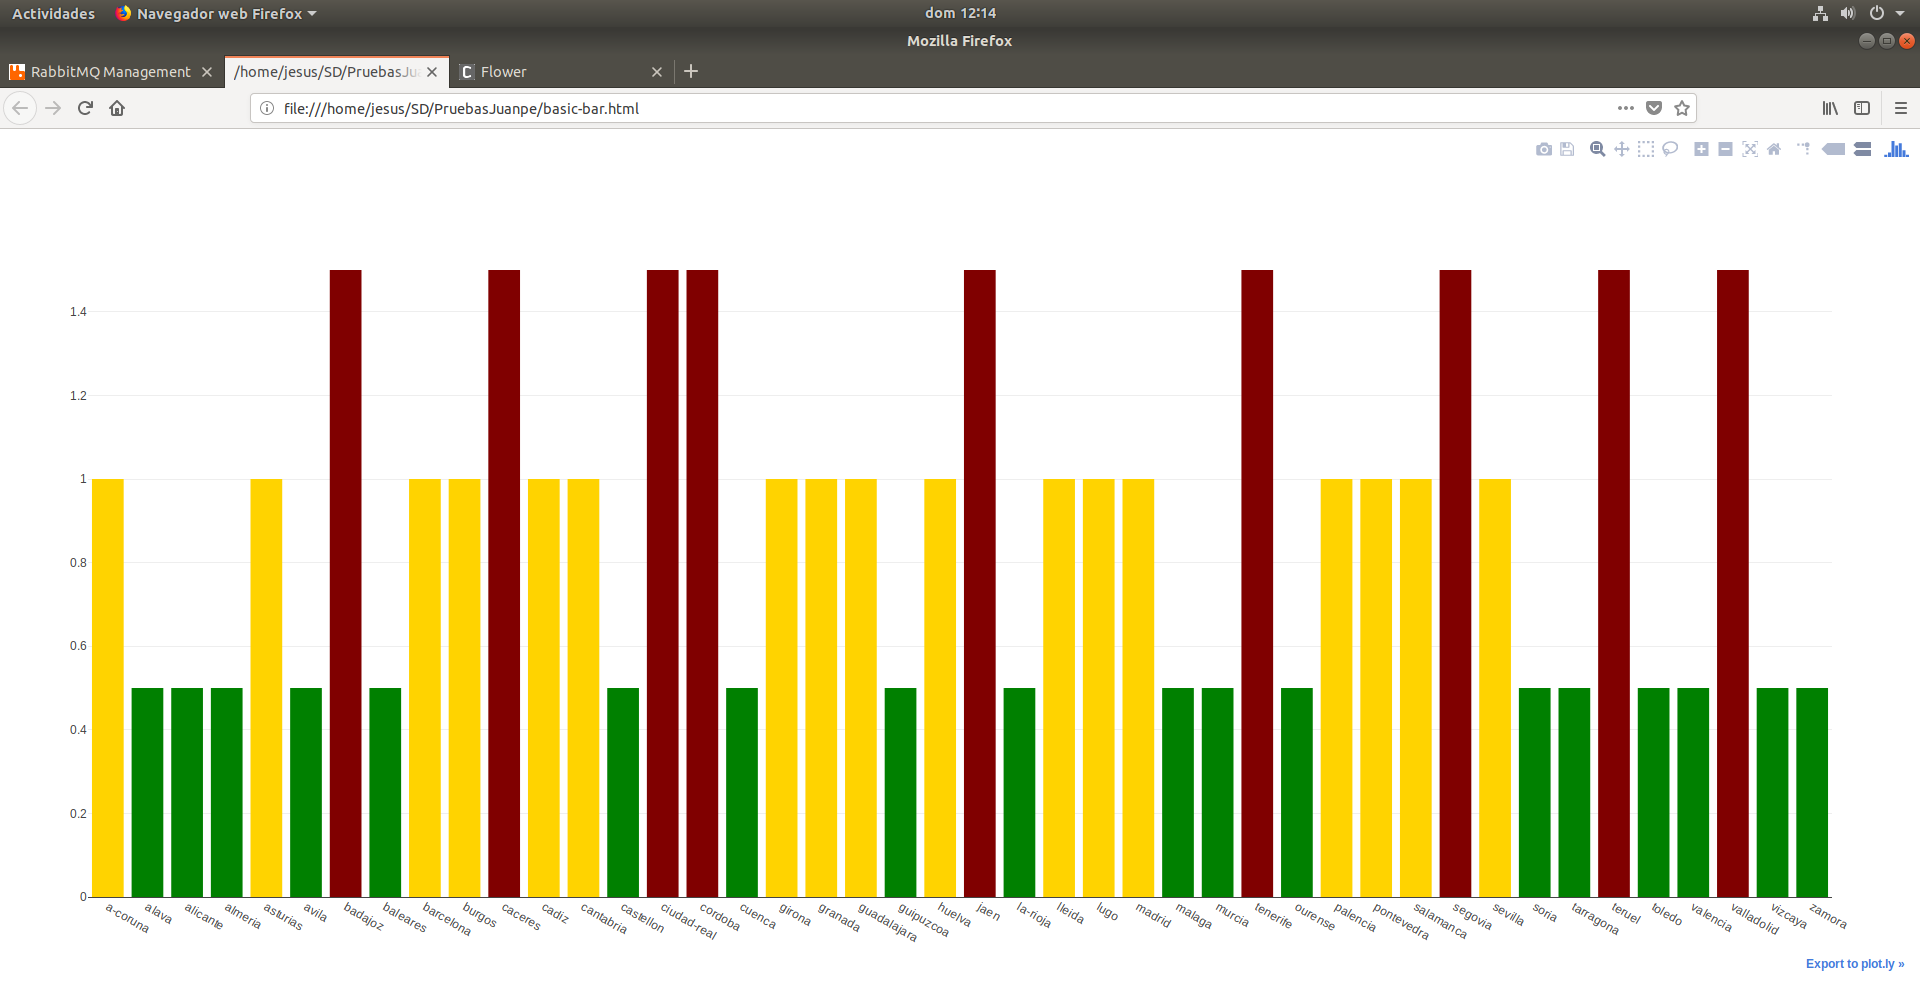
\includegraphics[scale=0.24]{5.png}
\end{center}

\begin{itemize}
	\item Resultado en Dropbox de la ejecución de \texttt{tareas.py} (cada minuto en las pruebas, pero la finalidad es cada una o dos horas):
\end{itemize}
\begin{center}
	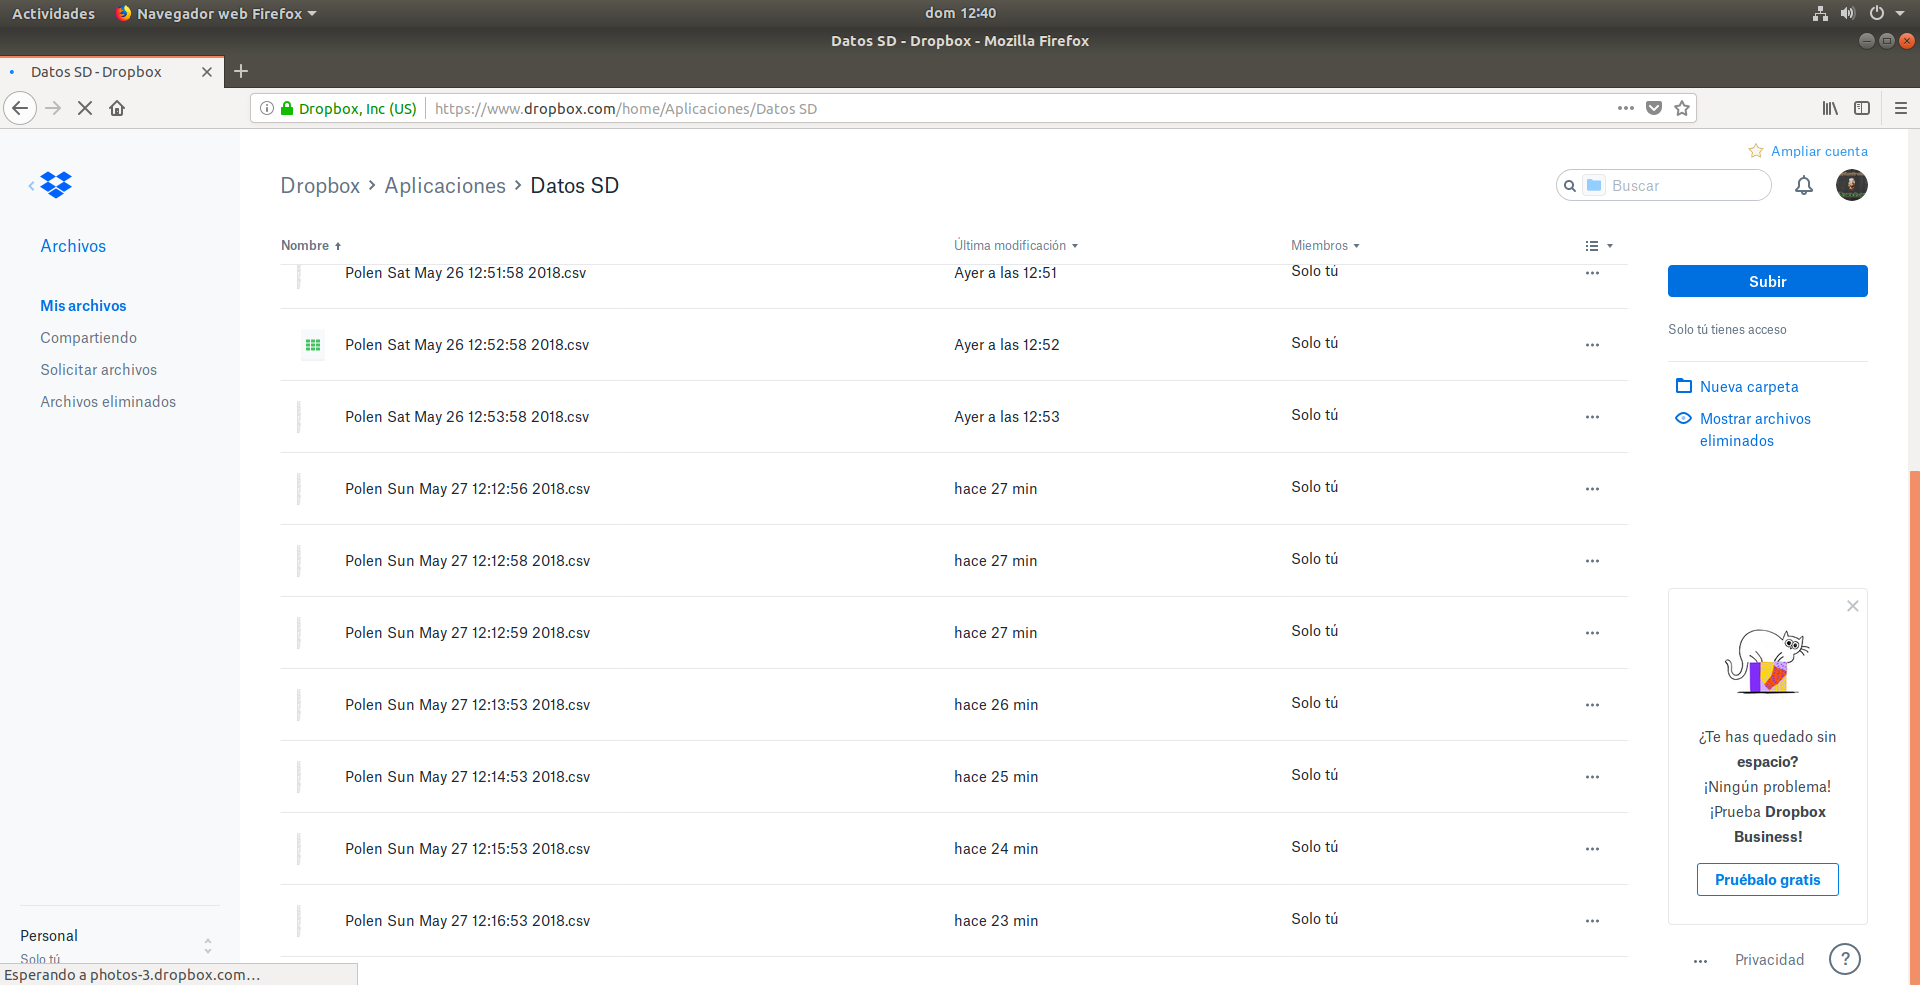
\includegraphics[scale=0.24]{8.png}
\end{center}

\newpage
\begin{itemize}
	\item Uso de \texttt{PolenCiudad.py} por parte de un usuario:
\end{itemize}
\begin{center}
	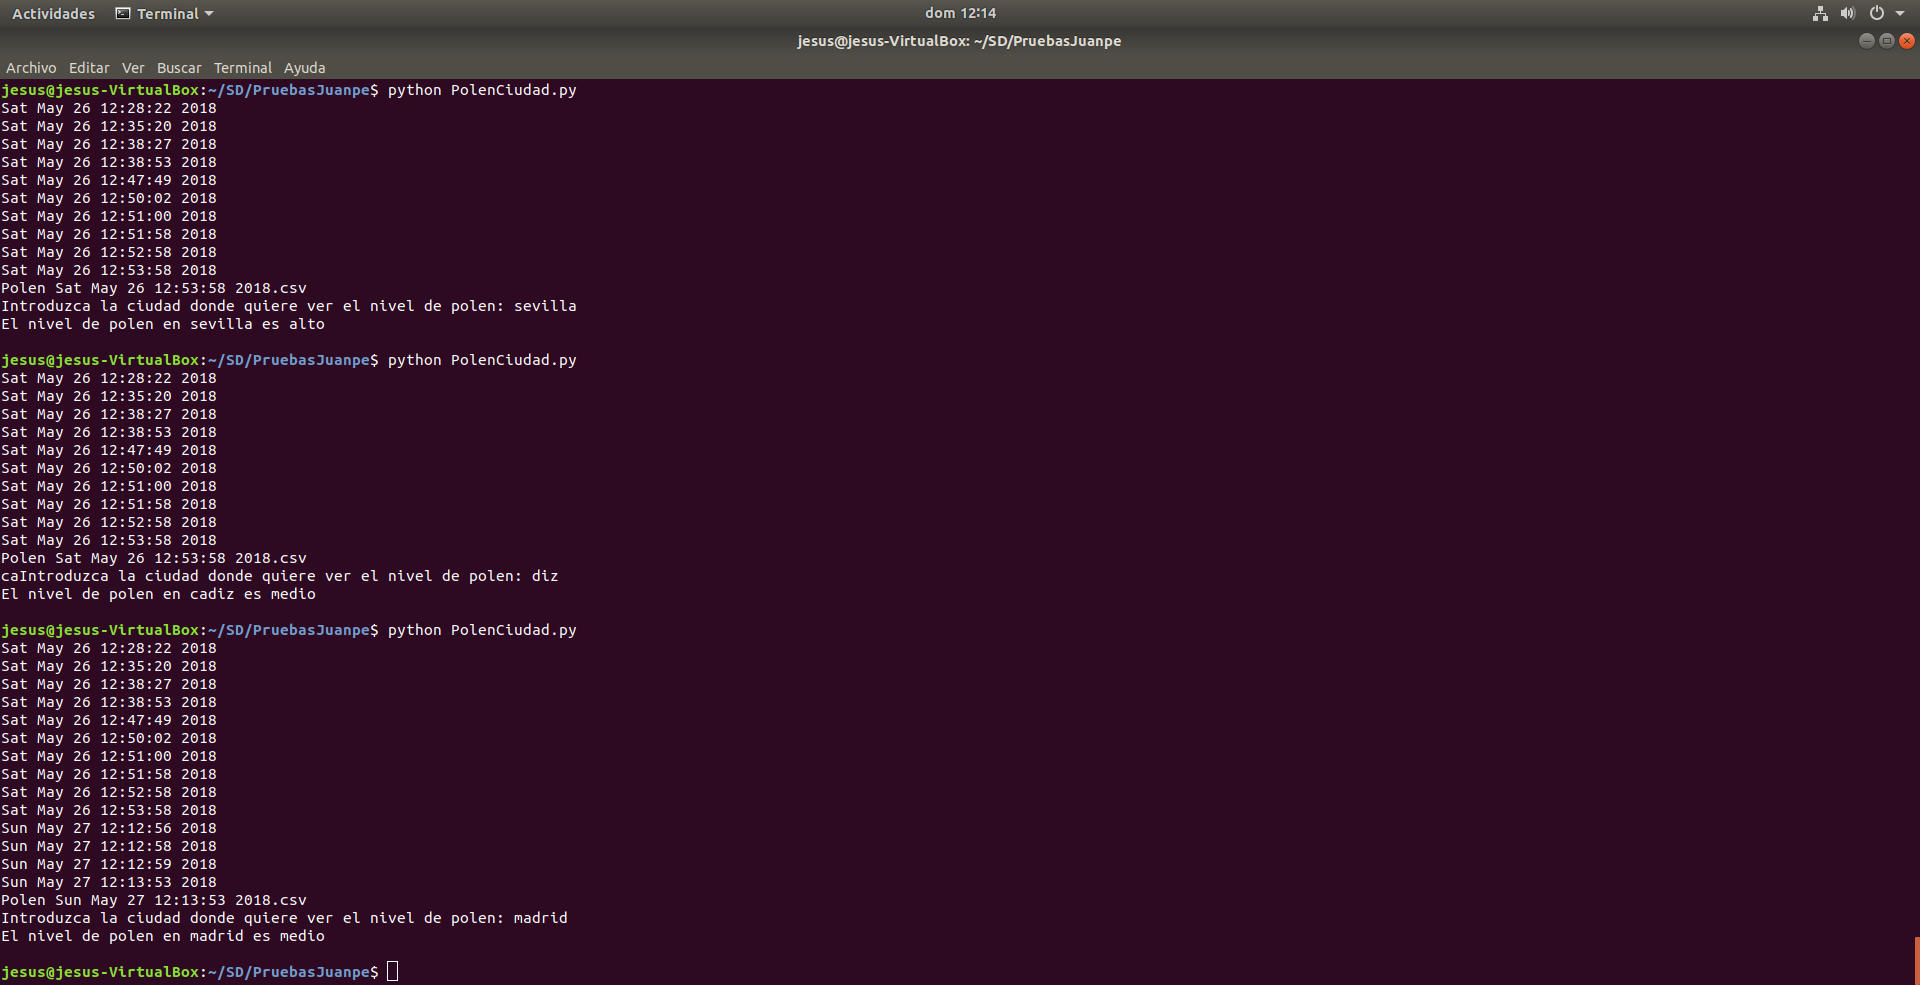
\includegraphics[scale=0.24]{6.png}
\end{center}

\begin{itemize}
	\item Resultados en twitter generados por la búsqueda del usuario:
\end{itemize}
\begin{center}
	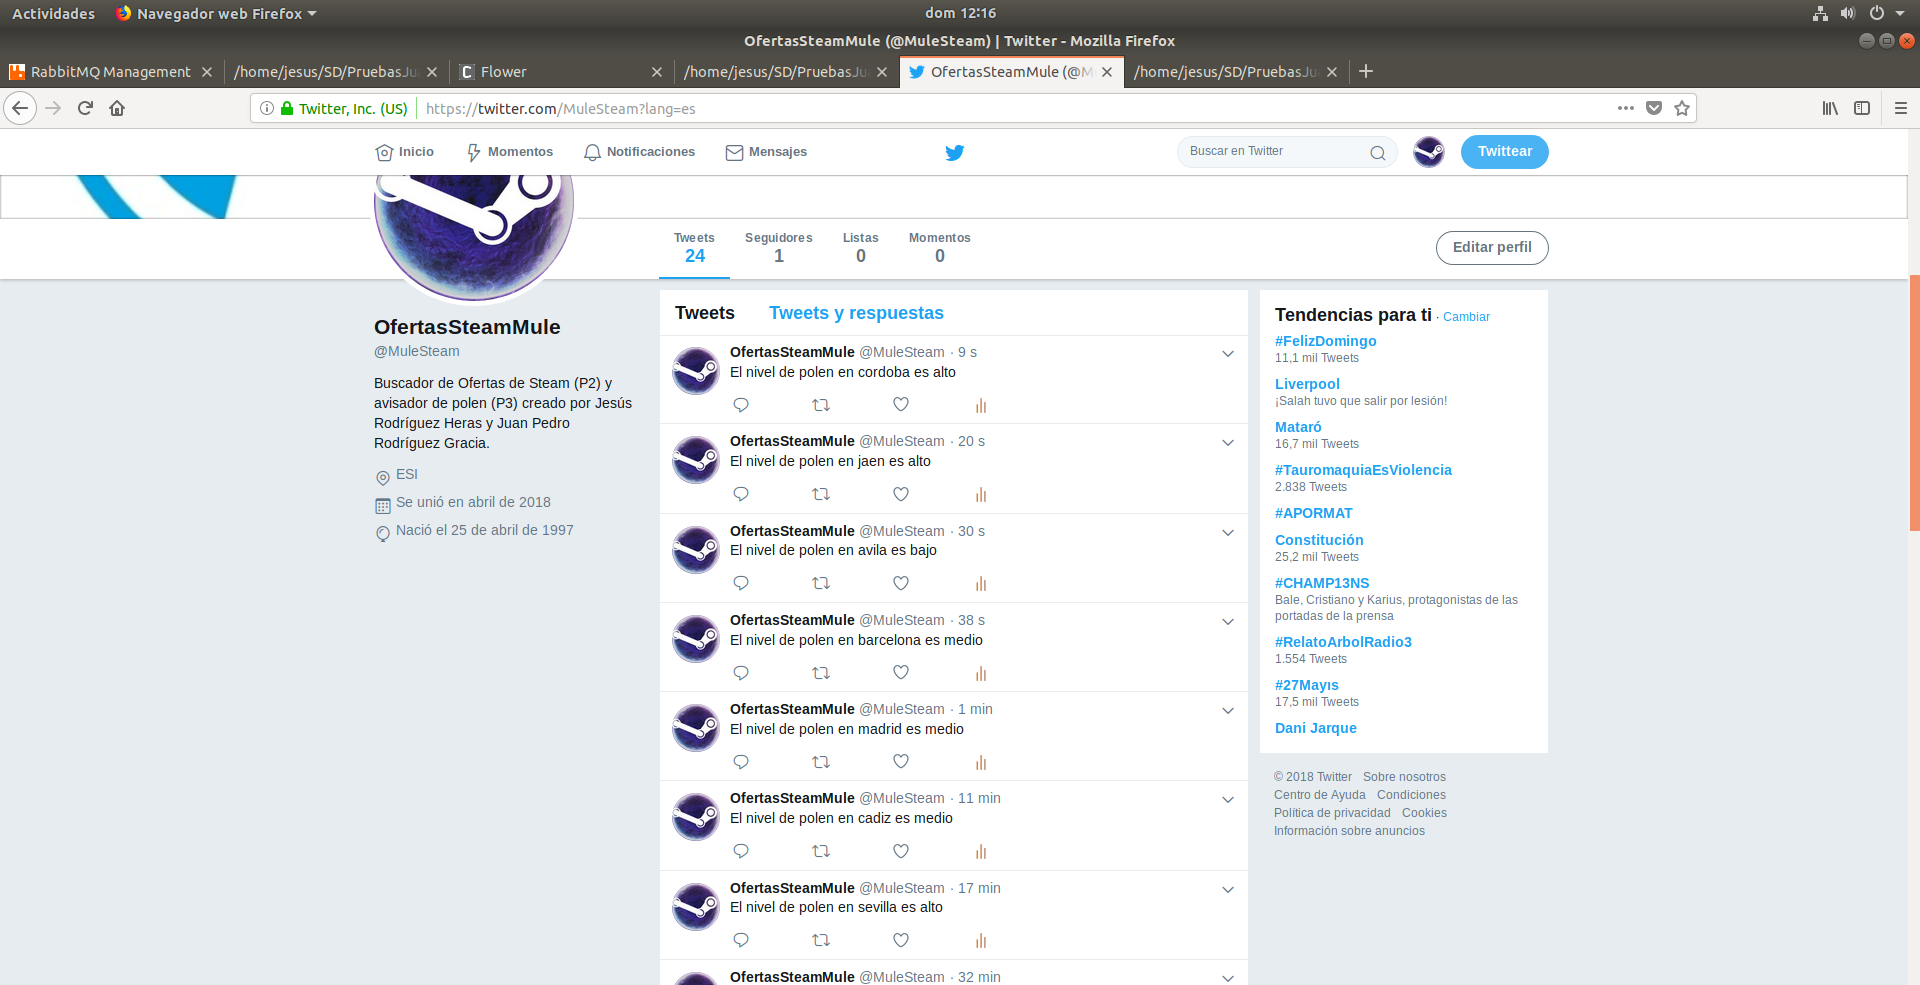
\includegraphics[scale=0.24]{7.png}
\end{center}



\section{Referencias}
\begin{itemize}
	\item \url{https://www.eltiempo.es/polen}
	\item \url{https://www.rabbitmq.com/}
	\item \url{http://www.celeryproject.org/}
	\item \url{http://flower.readthedocs.io/en/latest/}
	\item \url{http://dropbox-sdk-python.readthedocs.io/en/latest/}
\end{itemize}



\end{document}